\chapter{Our Daily Bread}
\vspace{0.6cm}
\begin{center}
\nopagebreak
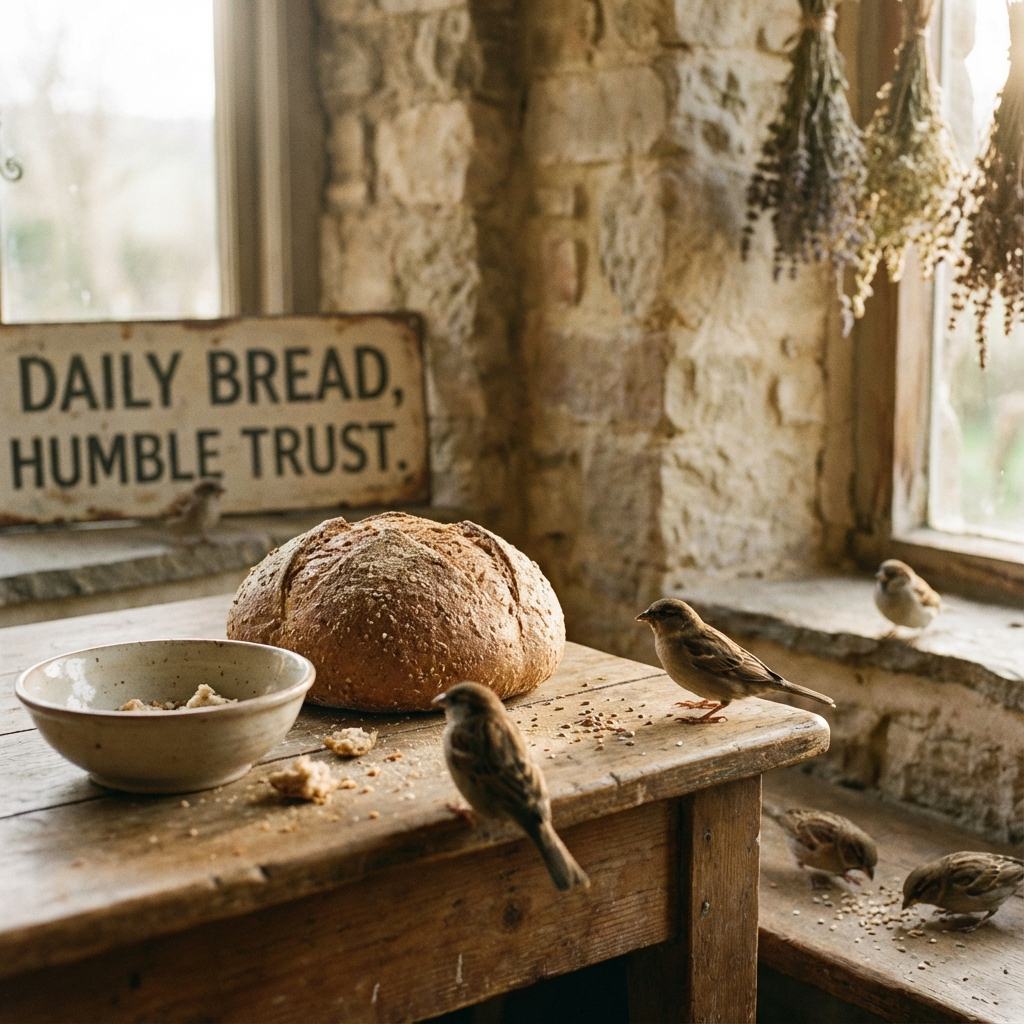
\includegraphics[width=0.75\textwidth,cfbox=gray!60 0.6pt 4pt]{bread_sparrows.png}\\
\vspace{4pt}
{\small\itshape Daily bread: absolute trust and spiritual nourishment.}
\end{center}

\vspace{0.6cm}
We were eating a calamari sandwich in Plaza Mayor. Jesus enjoyed it as if it were the most exquisite delicacy in the world.
—This is sacred —he said with his mouth full.


—The sandwich?


—The act of nourishing oneself. ``Give us this day our daily bread''.


He wiped himself with a paper napkin.
—People live with fear of scarcity. They accumulate, they store, they fear losing. That is a vibration of lack. When you ask for ``today's'' bread, you are trusting that tomorrow there will also be some.


—But one must be far-sighted...


—Being far-sighted is fine. Living distressed by the future is a lack of faith in Life. Look at the sparrows —he pointed to some birds pecking at crumbs—. They don't have granaries, and yet, they eat. Life sustains Life.


—And what about the people who have nothing to eat?


His face darkened a bit.
—That is not because bread is lacking. It is because selfishness is overflowing. If everyone vibrated in generosity, if everyone understood that we are one, no one would go hungry. The problem is distribution, not provision. The Universe is abundant. The human mind is what creates scarcity.


He took the last bite.
—The ``bread'' is also information, knowledge, love. Everything that nourishes you. Ask for what you need for today, to be your best version today. Do not ask to accumulate and feel secure. The only real security is your connection to the Source.